\documentclass[12pt]{article}
\renewcommand{\baselinestretch}{1.5}
\usepackage[utf8]{inputenc}

\usepackage{hyperref}
\hypersetup{linktoc=all}

\usepackage{amsmath}
\usepackage{amssymb}
\usepackage{listings}
\usepackage{color}
\usepackage{graphicx}

\definecolor{light-gray}{gray}{0.9}
\lstset{numbers=right,
                tabsize=1, 
					 numberstyle=\tiny,
                breaklines=true,
                showtabs=false, 
					 backgroundcolor=\color{light-gray},
                numbersep=5pt,
                xleftmargin=.4in,
                xrightmargin=.4in}


\usepackage{algorithm2e}
\usepackage{graphicx}
\usepackage{float}

\begin{document}

\title{Parallel Processing Final: \\Gaussian Elimination}
\author{Sarah Peachey \& Nathan Schomer}
\maketitle

% TODO: add abstract

\section{Design}

Gaussian Elimination is performed in two major steps:

\begin{enumerate}
    \item{Division- each element to the right of diagonal is divided 
        by the diagonal element.}
    \item{Elimination- for each diagonal element $k$, all elements below
        and to the right of the diagonal are reduced by the product
    of the elements at the projection onto both row $k$ and column $k$}
    \begin{itemize}
        \item{Note- during this step the diagonal elements are set to $1$
            and all elements below row $k$ in column $k$ are set to $0$}
    \end{itemize}
\end{enumerate}

These steps are performed $K$ times where $K$ is the width
(or height since the matrix is square) of the matrix. 
Due to issues discussed later, the zeroing of the sub-diagonal
was separated into its own CUDA kernel.

\pagebreak
\subsection{Division Step}

The division step contains no inherent dependencies between 
elements as they are divided by their corresponding diagonal
element. Because of this independence, this step can be fully
parallelized as long as the number of elements does not exceed
the number of available CUDA threads. In the case of a matrix
whose size exceeds the number of threads, striding will have to 
be used.

As seen in the code snipped below, the element A[k, tid] is 
divided by the diagonal element at A[k, k]. This opeartion
is performed for all elements in parallel.

\vspace{0.25cm}
\lstinputlisting[language=C, firstline=13, lastline=15, numbers=left]
{../gaussian_elimination/gauss_eliminate_kernel.cu }

\pagebreak
\subsection{Elimination Step}

The elimination step was parallelized for each element below
and to the current diagonal element A[k,k].
As seen below, thread (0,0) sets the current diagonal element 
A[k,k] to 1. This introduces a very minor amount of thread divergence.
This delay is minor especially since no threads have to wait
for this assignment to happen.

\vspace{0.25cm}
\lstinputlisting[language=C, firstline=28, lastline=29, numbers=left]
{../gaussian_elimination/gauss_eliminate_kernel.cu }

Next, all the threads, execute the code snippet below
which performs the elimination operation using striding if necessary.

\vspace{0.25cm}
\lstinputlisting[language=C, firstline=32, lastline=40, numbers=left]
{../gaussian_elimination/gauss_eliminate_kernel.cu }

\pagebreak
\subsection{Zeroing Sub-Diagonal Elements In Column K}

Finally, the sub-diagonal elements in column $k$ are set to $0$.
This operation was put in a separate kernel because it was necessary
to ensure all threads were done accessing these elements before they
were set to $0$ and ''\_\_threadsync()'' only synchronizes threads in
the current thread block. This grid-wide synchronization happens
by returning from the elimination kernel and calling 
''cudaThreadSynchronize()'' before calling the kernel to zero-out
the sub-diagonal elements in column $k$. As seen in the code 
snippet below, the threads stride in the column if necessary.

\vspace{0.25cm}
\lstinputlisting[language=C, firstline=45, lastline=50, numbers=left]
{../gaussian_elimination/gauss_eliminate_kernel.cu }


\pagebreak
\section{Results}
\vspace{-0.25cm}

\subsection{Discussion of Speed-Up}

Substantial speed-up was gained by the GPU version of the
Gaussian elimination algorithm. The Speed-Up was calculated 
using Equation 1. As expected, this speed-up increased as
the size of the matrix increased. Gaussian elimination
did not gain as much speed-up as some other algorithms.
This is partially due to the repeated access of global 
memory which is a burden on the speed of the kernel.

\begin{equation}
    s = \frac{t_{serial}}{t_{parallel}}\label{eq1}
\end{equation}

\begin{table}[H]
\centering
\begin{tabular}{@{}|l|c|}
\hline
Matrix Size & Speed-Up \\ \hline
512  &  4.23   \\ \hline
1024 &  14.04  \\ \hline
2048 &  42.26  \\ \hline
\end{tabular}
\caption{Speed-Up calculated on Xunil-05}
\end{table}

\subsection{Discussion of Error}

When compiling and executing our code, you may notice that
the program does not report ``PASSED''. After more than a
week of debugging time has run out and we need to examine
why the algorithm is not working properly. To visualize
the problem, the differences between corresponding elements
in the reference and the result matrices were written to
a third matrix. This difference matrix was then plotted
in a 3D surface plot as seen in Figure 1, Figure 2 and Figure 3.
Note- these plots are upside down so the error is located near
the last column and last row of the difference matrix.

All 3 figures show the majority of the differences between
the two matrices were zero or near-zero with the exception
of a few spikes. These spikes of error are concentrated 
near the bottom right of the matrix, above the diagonal.
Initially, it was hypothesised that the error was due to aggregation
of single-precision floating point rounding errors. However,
the error remained after changing all of the GPU calculations to
double-precision.

\begin{figure}[H]
    \centering
    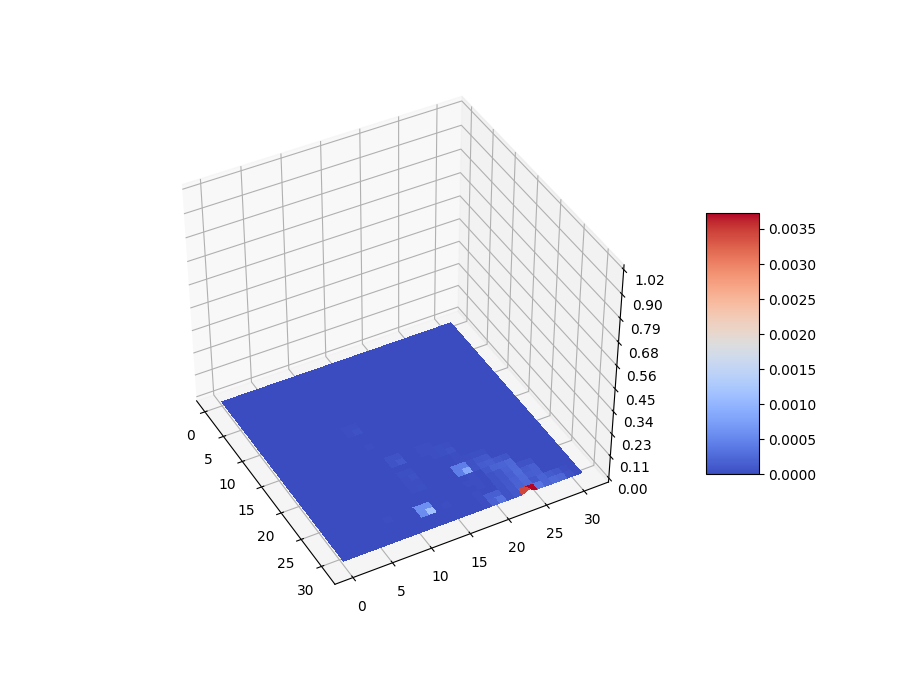
\includegraphics[width=\textwidth]{imgs/32.png}
    \caption{Difference for 32x32 Matrix}
\end{figure}


\begin{figure}[H]
    \centering
    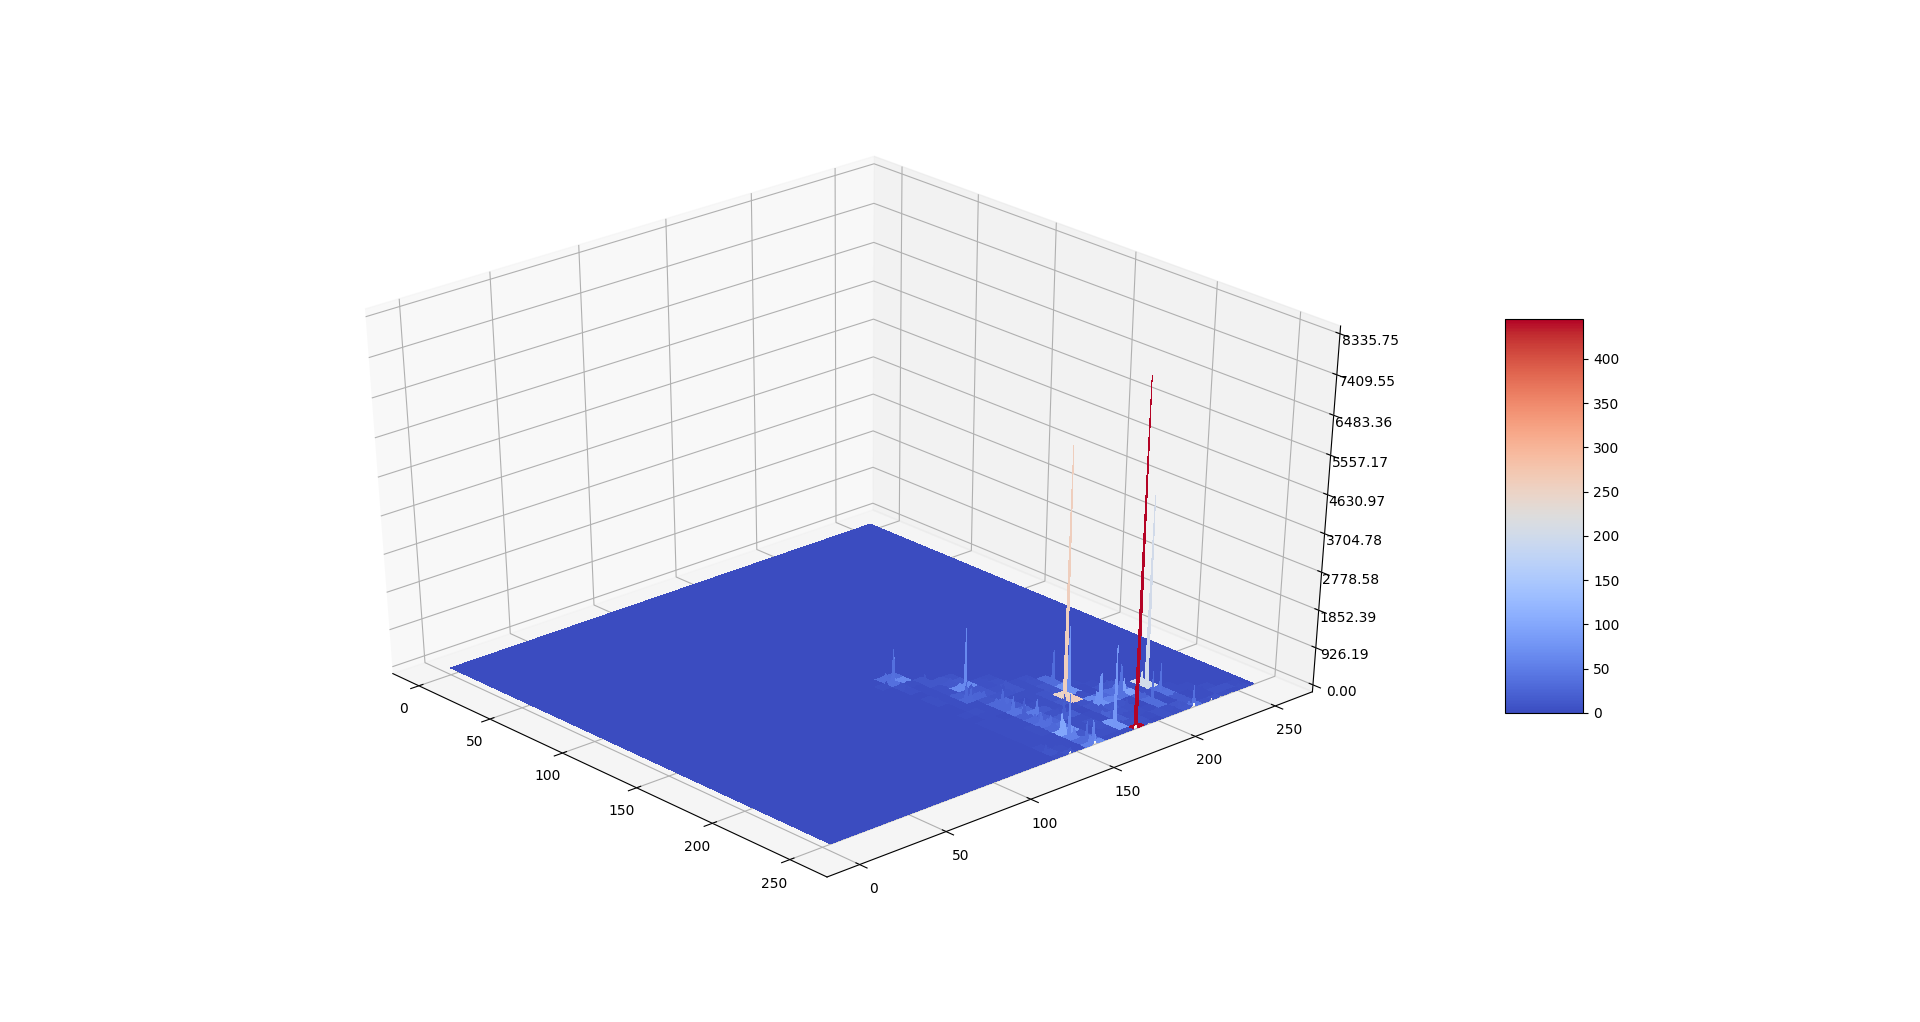
\includegraphics[width=\textwidth]{imgs/256.png}
    \caption{Difference for 256x256 Matrix}
\end{figure}

\begin{figure}[H]
    \centering
    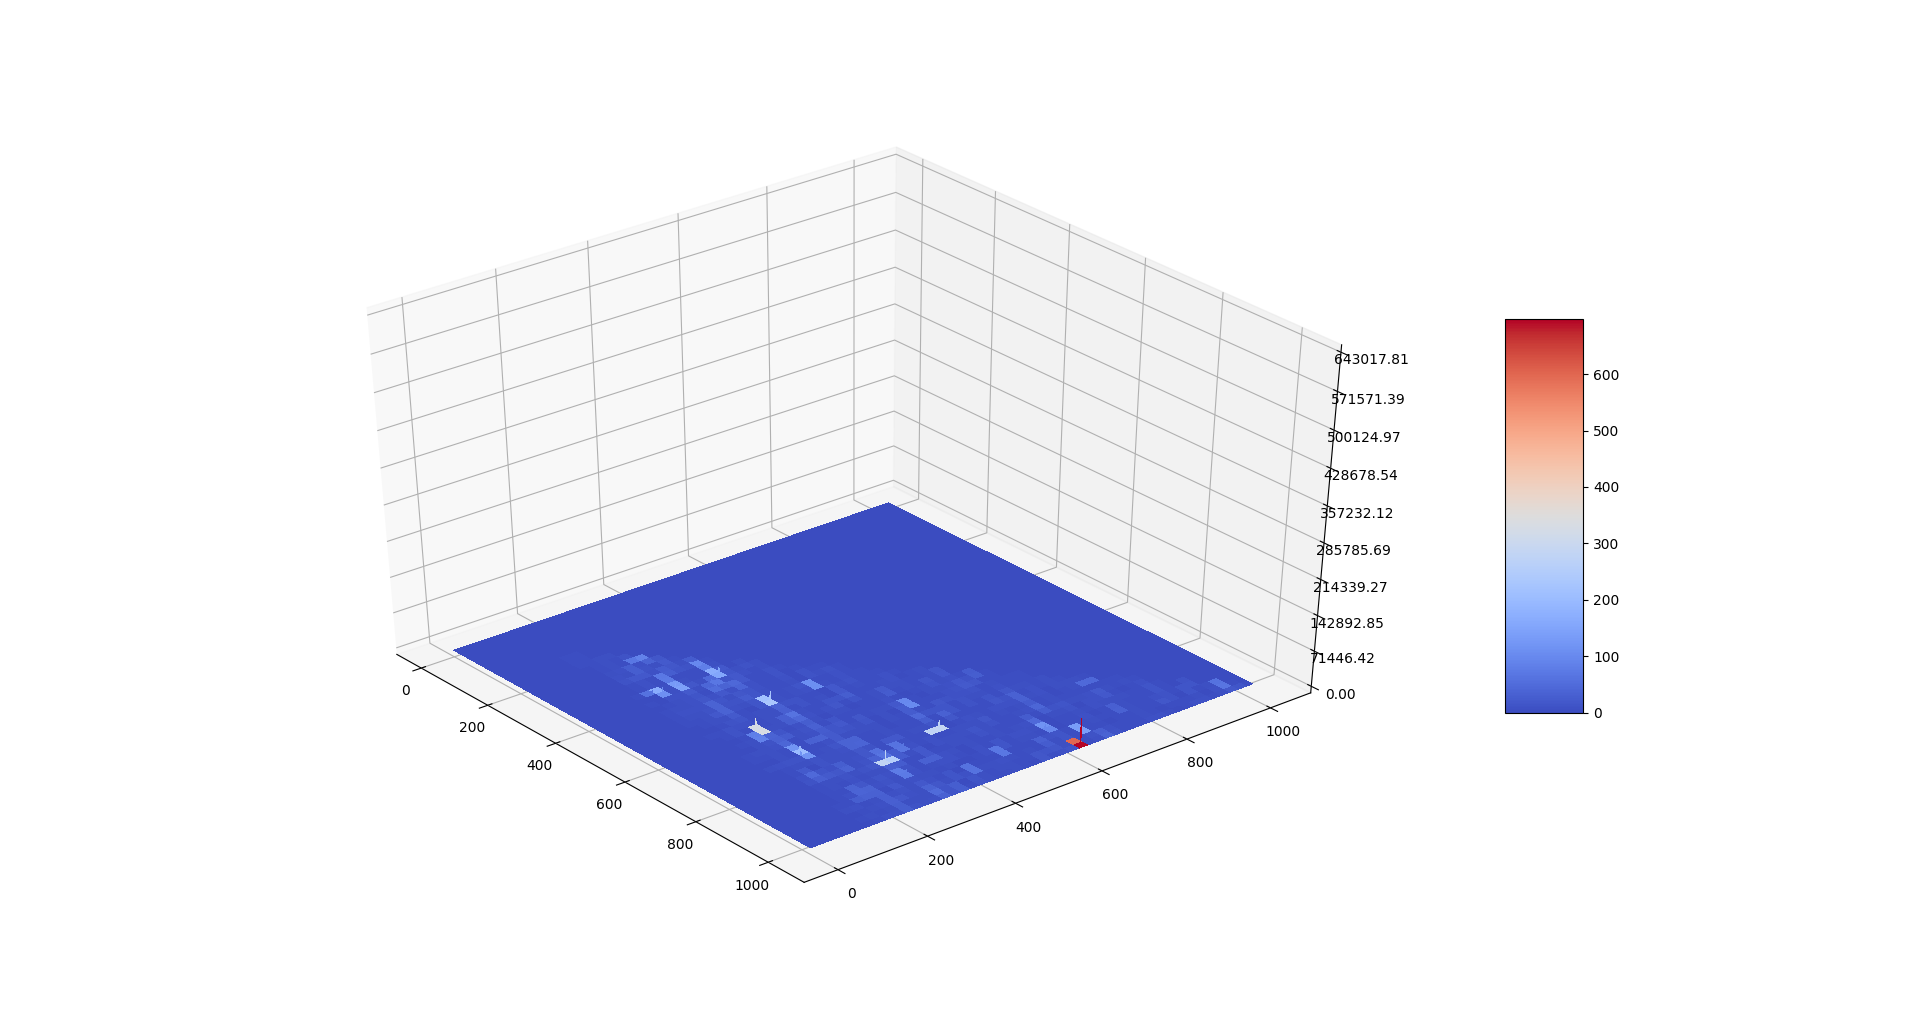
\includegraphics[width=\textwidth]{imgs/1024.png}
    \caption{Difference for 1024x1024 Matrix}
\end{figure}

\end{document}
